\chapter{Related work} % Main chapter title

\label{Chapter 3} 

\lhead{Chapter 3. \emph{Related work}}
% separer chaque system

\section{Introduction}
\par The idea of reusing an existing plan instead of planning from the scratch is not a new idea. Thus, we found in the literature many works from several researches who were interested by developing planning systems that include plan repair and replanning capabilities to deal with any unexpected events, while the plan is executed in a real-world environment. Most of these works were based on two approaches; the first is to build an additional structure with the produced plan to help the planner in the replanning phase. The second approach uses a planning heuristic to choose the most promising tasks to refine. 
In this chapter, we discuss the most recent of these approaches. 

\section{Approaches based on additional structures}
 The systems presented in this section, construct with the solution plan, an additional structure which brings more knowledge in order to help the planner repairing the breakdown. 
 
\subsection{Replan system}
\par The first system presented is \textit{Replan} system \cite{boella2002replanning}.The HTN formalism used for this system is an extension of the declarative planning HTN formalism.
The task architecture used in \textit{Replan} is based on two hierarchies. On one hand, the \textit{sequential abstraction hierarchy} that contains complex tasks. These tasks type subsume more primitives one. On the other hand, the\textit{ abstraction hierarchy }which is a task decomposition hierarchy such that a task type can be substituted with a sequence of tasks, this type of task is called abstract task. The definition of actions was also augmented, in fact the action’s effects are composed by effects of the action when the preconditions of the action hold and the effects of the action when its precondition do not hold. 

In addition, each task in the \textit{Replan} system has an utility interval which express the upper and lower bounds of the best and the worst outcomes by refining the defined task. The produced utility is used to choose the best decomposition when refining (decomposing) a task.


The planner starts the decomposition from the top goal task and at each refinement step, the planner computes the expected utility of a partial plan generated by projecting it from the current world state, afterward a pruning heuristic is used to eliminate all the suboptimal plans that have their utilities dominated by some other plan. For the resulting plan, \textit{Replan} constructs a derivation tree that describes how the plan was derived and includes all the tasks involved in the construction of the plan. This tree is essential for the plan recovery process.

 
During the execution process, a breakdown is identified in the case where the plan doesn't reach the goal or that it reaches with a very low utility compared to what was expected in the planning process.
The replanning algorithm is based on a \textit{partialization} process. The partialization process starts by finding the leaf node in the derivation tree whose preconditions do not hold in the current world. This action is marked as focused action (FA). 
If the FA is subsumed by an abstract task, then the FA and the abstract task are removed from the derivation tree. However if the FA appears in the decomposition of a complex task, then the planner will search for a descendant of a sibling node of FA which has not been executed yet, if the action exists, this later will be marked as the current FA. 
However, if all the siblings of the FA have been refined, then all the siblings and the FA are removed from the derivation tree, and the parent complex task become the current FA.
The partialization process stops when a promising plan is found, in the worst case the whole derivation tree is discarded.  A promising plan is a partial plan that has higher bound utility than the old one. Otherwise the partial plan is discarded. The promising plan is then refined to achieve the goal.  

\subsection{HOTRiDE system}
The next system we present is built on the top of a famous HTN planner \textit{SHOP}\cite{nau1999shop} and attempts to help the planner  recovering from  plan failures. 


\textit{SHOP} is an HTN domain independent planning algorithm , which make a constraint that tasks must be planned in the same order that they will be later executed. Thus the decomposition produced by each method has to be a total ordered set of subtasks. This constraint gives SHOP knowledge about the current state at each planning step which improves its degree of expressive power in its knowledge base. Nevertheless, as plans are computed in off-line phase, the world can change and causes breakdowns.

 
In order to rectify this situation, a plan repair system proposed. This later is built on the top of a modified version of SHOP and its called \textit{HOTRiDE} \cite{ayan2007hotride}.

HOTRiDE is a planning system, (Hierarchical Ordered Task Deplaning in Dynamic Environments), which provides plan generation, execution, and plan repair system to recover from breakdown situations. 


The planning process is based on SHOP planning algorithm, in addition to the resulting plan, \textit{HOTRiDE} produces a task-dependency graph that consists of HTN traces generated by the planner  representing the dependencies between the tasks using causal links.

\textbf{Causal link (a, t):} a causal link between two task t1 and t2 is a pair (e, p). 
\begin{itemize}
\item[-]In case where t1 and t2 are primitive tasks, then e is an effect of t1, and p is a precondition t2.
\item[-]If t1 and t2 are compound tasks, then e is the effect of sub-action generated by decomposing t1 and p is a precondition of t2. The causal link (e, p) means that the task t1 supports the task t2.
\end{itemize}


An HTN trace for a task t consists of an ensemble of HTN trace nodes where each HTN trace node is defined as a tuple \textit{N= (t, $\pi$, A, D, Q, C)} where t is a task, $\pi$ is the plan that achieves the task t. A is a cumulative addition to the current state resulting from achieving the task t and D is the cumulative deletion made to the state while achieving the task t. Q represents the preconditions of t. and C is a  set of pointers to the child nodes of the node N.
A task-dependency graph is represented as triple $DG = (DT, CL, PL)$. Where:
\begin{itemize}
\item$	DT$: HTN trace.
	\item $CL$: causal link list: for every p ground atom, CL(p) is an ordered list of heads of ground operator instances that add (delete) p to (from) the state. 
	\item $PL$: is a totally ordered list of all the tasks that have a ground atom p as a precondition. 
\end{itemize}


Once the task dependency graph is computed, the plan is passed to the controller for the execution process. As the environment is dynamic, the controller monitors the current state at each execution step, and tries to execute the action step in this current state.  If at any point the controller detects a breakdown, \textit{HOTRiDE} identifies the failed action i.e the action whose execution cannot end in the current state.  Then \textit{HOTRiDE} starts the recovery process.

The recovery process starts by first, checking every parent of the failed action using the task-dependency graph to identify the minimal failed parent. 
The minimal failed parent is either a compound task that is identified as failed but whose parent is not, or a goal task that does not have any parents in the task-dependency graph.

For example, during the execution of a plan (see Figure.\ref{Dependency graph}), the execution of the action D failed, \textit{HOTRiDE} traverses the hierarchy of the task-dependency graph in the upside-down manner to detect the minimal failed parent task of the action D. 
Once the minimal failed task; in the example A2 is detected, \textit{HOTRiDe} detects the set of all causal links supported by the initial plan.
If the task A2 is not the first descendant of its parent, then \textit{HOTRiDe} marks only A2 as minimal failed parent and invokes SHOP to generate a new decomposition for A2 and its corresponding dependency graph. 
Next, HOTRiDE establishes all  the causal links between any task of the new dependency graph and the tasks in the previous dependency graph that are not accomplished yet. 

Nevertheless, if SHOP cannot find a new decomposition for A2, or all the decompositions found fail then, \textit{HOTRiDE} marks A2 and its parent A as failed tasks, and attempts to replan for A.

\begin{figure}[h]
	\centering
	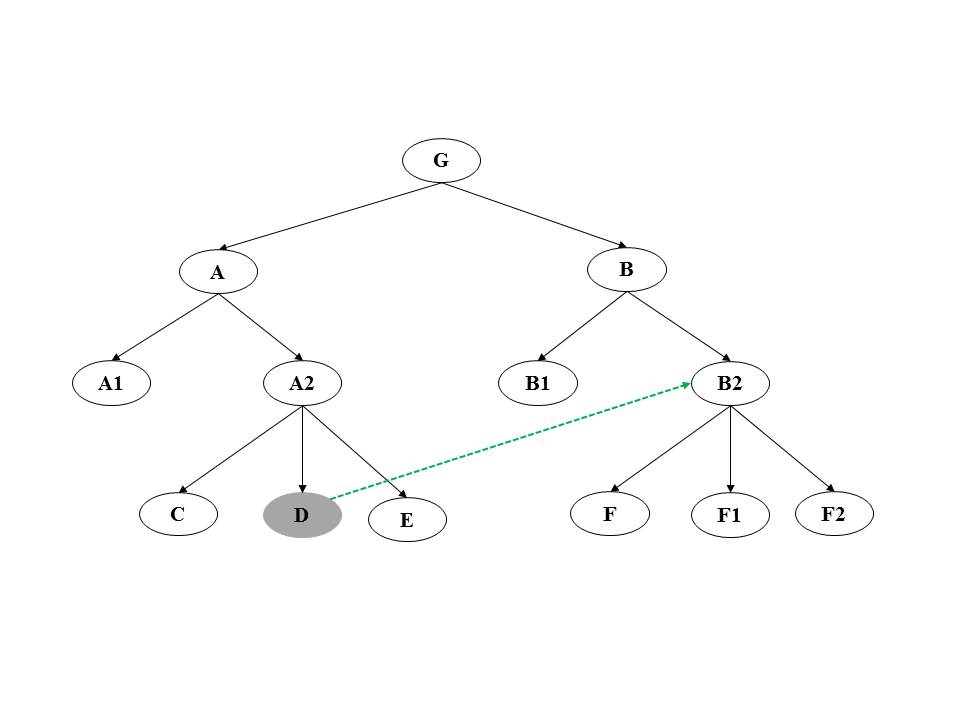
\includegraphics[width=0.75\textwidth]{Pictures/hotride.png}
	\caption{\label{Dependency graph} Dependency graph example}
\end{figure}

After replanning, there may tasks in the original dependency graph that are no longer supported by the new plan. For example the task B2 was supported by D in the original plan; if the task is no more supported, then \textit{HOTRiDE} marks it as failed task and attempts to generate other decompositions for it. If there is no such decomposition, \textit{HOTRiDE} tries other possible decompositions for the minimal failed parent task A2.

This process is repeated for every causal link not supported in the new plan until SHOP generates a new plan that satisfied all the causal links. \textit{HOTRiDE} executes the new plan starting from the failed action D in the current state of world.  Otherwise \textit{HOTRiDe} repeat the plan repair on the hierarchy of the parent of D until one of the following holds; HOTRiDE generates a plan that is executed successfully in the world; or in the worst case, the plan repair process marks a goal task as failed and replans from the scratch. 

\subsection{repairSHOP system}

As \textit{HOTRiDE}, \textit{repairSHOP} is also built on top of a modified version of SHOP  \cite{warfield2007adaptation} and uses the same approach. However, the tow systems differs in the structure of the tree used in the repair plan process. 


RepairSHOP augments the planning system SHOP with a direct goal graph (GG) to allow SHOP with replanning capabilities.  The Goal Graph uses a Redux architecture that combines the theory of Justification-based Truth Maintenance System (JTMS) and Constrained Decision Revision (CDR). This combination provides the ability to the GG to perform dependency-directed backtracking in order to propagate changes when a failure occurs.  


JTMS is a dependency tree where nodes are called assertion. Each assertion is associated with a justification  composed of two lists of assertions. The first is IN-list and the second is OUT-list. The assertions in the IN-list are connected via “+” links, while those in the OUT-list are connected by “-“ links. The valuation of assertions depends on the validation of its justification. 

A Justification is valid if every assertion in the IN-list is labeled IN and every assertion in the OUT-list is labeled OUT. A believable assertion is labeled IN and in contrary an assertion that cannot be believed is labeled “out”. 


The GG is composed of goals, decisions and assignments. A goal might be performed by several recipes called decisions. The role of a decision is to decompose a goal into a set of sub goals, in addition each decision contains a task list that contains the decomposition of the performed goal and an assignment list that contains the conditions needed to perform the decision on a goal. The goal is represented by tasks in SHOP and assignments are the preconditions and the order constraints of tasks.

The GG is computed automatically during the planning process as follows: 
\begin{itemize}
\item	Each task is encapsulated in a goal structure in the GG
\item primitive task successfully planned is added to its parent  goal list
\item	The planner considers each possible decomposition for each compound task and encapsulates this reduction with its conditions in a new decision. If the task decomposition succeeds then the plan is added to the decision’s goal list and the GG marks the additional decompositions left not evaluated as \textit{NULL}. These decisions are used later in the plan recovery process. If the task evaluation fails then the decision is marked as OUT.
\item	RepairSHOP constructs justifications for branches where a failure may occur.
\end{itemize}
The controller starts the execution process and attempts to decompose each compound task G using its corresponding decision O. When a decision O fails to decompose a task Ti, the planner labels the decision O as invalid. Then the plan repair process starts. 


The controller check to see if alternate decision OG previously marked NULL is available to decompose the goal Ti this decision is labeled in the GG as valid decision. The GG is updated to records the modifications. Otherwise if any decision is found to decompose Ti then the controller backtracks in the GG to propagate the result to the highest affected goal and returns the first available alternate decision from the nearest goal node. If an alternate decision is found, the controller calls SHOP to replan from this goal. 


%In the next section we introduce another approach of plan repair based on use of a heuristic.
 
\section{An approach based on heuristics: Dynagent}
The system presented is an HTN forward chaining planner combined with an A* like heuristic search, to plan, execute and adapt a robot plans in dynamic environment. This system is called \textit{Dynagent} \cite{hayashi2006dynagent}.


The planning algorithm proposed in this system is a forward HTN planner similar to the SHOP planner presented previously. In addition, this system extends the notion of the HTN’s components for the purpose of replanning. These compounds are called tasks plus, actions plus and plan plus.

For each task plus preconditions were extended to protected conditions and remaining conditions. The satisfiability of the protected conditions have been confirmed in the process of planning, and they will be used to detect the invalid plans when the belief is updated. The satisfiability of the remaining conditions remains to satisfy during the planning process. An action plus is considered as solved action plus if its remaining set is empty. 

In addition, each action plus records the initiation set and the termination set. The initiation (respectively, termination) set records the primitive fluents which start (respectively, cease) to hold after the action execution HTN planning \cite{hayashi2006dynagent}. 

The plan plus records two types of plans, solved plan plus which all actions that it contains are solved actions plus and supplementary plan plus is a plan which contains a task plus or action plus such that one of the fluent in its remaining set is marked as invalid. The supplementary plans are later used to generate new valid plans when the fluent becomes valid. 

The recipes used to refine tasks are HTN rule for decomposing abstract task and actions rule that are used to process primitive actions or tasks. These recipes contain the preconditions that must be satisfied before refining a task plus and action rules. Each task has an estimated cost from refine it and the cost of a plan is the sum of each cost of task in this plan.

The agent starts observe the current world at each stat and update the belief as follows:
\begin{itemize}
\item[-]If a fluent is deleted then the planner deletes all the invalid plans from the current set of plans and the set of supplementary plans. 
\item[-]Otherwise, if a fluent is added, the planner make the new valid plans from the set of supplementary plans. 
\end{itemize}


The planning process starts by detecting all the applicable plans plus. Next an A* heuristic is called to choose the best plan plus to refine based on the cost of the actions composing the plan.

The planner proceeds to the refinement of the plan plus by decomposing the tasks in this plan and replace its occurrences in the current set of plans plus. This procedure is repeated until each remaining conditions of tasks involved in the current set of plans plus become empty.  The planner returns a solved plan plus and update the current set of plans plus and the set supplementary plans.
During the execution the belief is continuously updated to monitors the execution of actions in the plan. 
Thus, when an action execution is successful it executes the following procedure 
\begin{itemize}
\item[-]	Delete from the current set of supplementary plans plus all the plans plus whose first element is not a solved action plus.
\item[-]	The fluents in initiation set of the executed action are added to the current belief and the fluents in the termination. 
\item[-]	After the belief update, the planner deletes all the invalid plans plus from the current set of plans plus and the current set of supplementary plans.
\end{itemize}
Otherwise, when an action execution fails then the controller deletes each plans form the current set of plans plus and the current set of supplementary plans that contains an action which is unifiable with the failed action.  

%%We have presented an agent system combining forward chaining HTN planning, A*-like heuristic search. This system uses A*-like heuristics for selecting the task to be decomposed, which is different from our solution that  aim is to define a classical planner that can be used to recover from the breakdown.
\section{Conclusion}
We presented in this chapter plan repair systems which are based on partial replanning from the initial domain. Theses systems prove their efficiency on different real planning problems. Nevertheless, they present certain limitations. First,  the plan repair approach followed  is depended to the initial planner. If the latter is unable to find new decompositions for the failed tasks, then the  plan repair algorithm will return no solution and the plan execution will fail.
 Second, these systems assume that modeling a complete domain knowledge is possible, but as the domain knowledge is always incomplete (see chapter \ref{Chapter 2}), then the plan repair (based on a dependency graph itself probably incomplete, or using a heuristic on an incomplete domain) will very likely lead to a new breakdown. The system will therefore never reach the goal state. In addition the use of a heuristic requires a declarative formalism of tasks to evaluate them. Thus, we consider that  the proposal  do not offer a flexible approach to tackle the incomplete definition of reactive HTN's domain knowledge. 
  
 In the next chapter, we will present our proposition for a recovery planning system that can recover from breakdowns in reactive HTN with incomplete model. 






 
